\section{提升推理模型鲁棒性的数据增强策略}

在人工智能领域,常识性推理作为一项核心任务,其挑战在于赋予机器与人类相似的理解和决策能力。
尽管神经网络模型如BERT\cite{devlin2018bert}和RoBERTa\cite{liu2019roberta}
在ROC\cite{mostafazadeh2016corpus}、
COPA\cite{roemmele2011choice}、ARCT\cite{habernal2018argument}和RECLOR\cite{yu2020reclor}
等任务上取得了显著成就,它们在处理对抗性数据或不同于训练环境的场景时仍显脆弱。
这种局限性通常源于模型对数据集中特定模式的过度依赖,而非深入理解问题本
质\cite{naik2018stress,mccoy2019right,schuster2019towards,nie2020adversarial}。
在上一章对模型鲁棒性差的原因的解释中我们也验证了的确受到偏差数据的影响。

针对模型鲁棒性不足的问题,本章提出了一种数据增强方法,旨在提升常识性推理模型的鲁棒性。这
种方法通过创新的数据增强手段减少数据的简单统计偏差,从而增强模型的鲁棒性。

本研究的灵感来源于生物
学中的``交叉''和``变异''过程。这一策略模仿生物遗传中的染色体交叉和基因变异,
创造问题实例之间的新组合和变化。``交叉''操作涉及交换两个不同问题的选项,
而``变异''操作涉及对问题的某些部分进行微妙修改。这些操作产生新的、具有挑战
性的训练实例,促使模型超越表面的统计规律,深入学习问题的内在逻辑和结构。

这些策略被应用于领先的神经网络模型,并在多个基准数据集上进行
测试。实验结果显示,这些策略显著提高了模型在多样化和对抗性数据环境
中的鲁棒性,同时在标准测试集上保持或提升了性能。


\subsection{概述}
\label{sec3:intro}
选择题(MCQs)是一种常用的格式,
用于评估自然语言理解(NLU)能力,涵盖了因
果推理~\cite{roemmele2011choice}、故事结尾预
测~\cite{mostafazadeh2016corpus,huang20story}、论
证理解~\cite{habernal2018argument}以及阅读理解~\cite{yu2020reclor}等任务。
这些任务通常由一个情境描述(前提)和几个选择项组成。
例如,COPA 数据集~\cite{roemmele2011choice}通过 MCQs 
来测试常识性因果推理~\cite{luo2016commonsense},一个典型的例子如下:

\begin{example}\label{ex:copa}
    COPA 选择题示例:
    \begin{description}
        \item[Premise:] The man hurt his back.
        \item[Choice 1:] He stayed in bed for several days. \checksymbol
        \item[Choice 2:] He went to see a psychiatrist. \crosssymbol
        \end{description}
        \end{example}

近年来的研究开始探究高级神经模型在 NLU 推理问题上的强大表现。
特别是,研究发现许多模型可能并不是通过真正理解上下文与选项之间
的逻辑和语义联系来取得成功,而是通过利用训练和测试数据中的偏见或
统计特征。这一观点得到了``仅选项测试''(也称为``仅假设测试'')的
支持~\cite{sharma2018tackling,bras2020adversarial}。在这种测试中,
模型如 BERT 在没有前提的情况下也能正确回答问题。

我们将这种现象称为自然语言推理中的``短路''。虽然``仅假设测试''为短路行为
提供了一些证据,但我们认为它具有一定的局限性。即使模型在没有前提的情况下
能正确回答问题,也不一定意味着它在有前提时不会考虑前提。

为了更全面地测试这种``短路''现象,我们尝试了一种新方法:绘制模型在处
理完整问题时,最后编码层中单词间的注意力图。如图\ref{fig3:att-goodex}所示,
我们使用了来自 COPA(见\exref{ex:copa})的示例。注意力图清楚地展示了,在处理
完整问题时,模型对于第一个选项与前提之间的联系几乎没有关注,而当仅处理选项,无上下文时,
选项内单词之间的注意力保持不变。

\begin{figure}[th!]
\centering
\includegraphics[width=0.5\columnwidth]{figures/ecai/end_related.eps}
\caption{展示 BERT\cite{devlin2018bert} 在 COPA 问题上短路的注意力图。}
\label{fig3:att-goodex}
\end{figure}

尽管使用注意力图来手动检查模型的短路行为可以提供洞察,但这
一过程既繁琐又成本高昂。因此,我们开发了一种自动化的白盒测
试算法,使用阈值来模拟人类的视觉过程。但这种方法也有局限性:它
需要访问模型的内部代码,并且只适用于基于注意力的模型。

为了解决这些挑战,我们引入了一种新操作,称为``交叉'',用于 MCQ 问题实
例。这种操作通过交换两个 MCQs 的选项来模拟生物繁殖中的染色体交叉过
程。这对经常利用短路行为的模型提出了独特挑战,通过构建代理测试案例
可以在真实任务中检测这种行为。我们在三个最新的、强大的 NLU 推理模型上
进行了这种交叉测试,发现这些模型在实例级别的压力测试中表现出明显的
准确率下降,显示出短路行为。

在确认了短路行为的存在后,我们的目标是提高模型的鲁棒性。我们考虑了
使用挑战模型难度的压力测试生成更多训练实例的方法。但由于许多压力测
试对选项构建有限制,这限制了它们作为通用数据增强方法的有效性。然
而,交叉操作及其对应的``突变''操作提供了一个可行的解决方案。这些操作
不仅可以用于检测短路行为,还可以作为有效的数据增强技术,减少短路行为
的发生,从而提高 NLU 模型的整体鲁棒性。
为此,我们应用
交叉、突变和反向翻译~\cite{xie2020unsupervised}来增强 BERT、XLNet~\cite{yang2019xlnet} 和 RoBERTa~\cite{liu2019roberta} 在 ROC~\cite{mostafazadeh2016corpus}、COPA、ARCT~\cite{habernal2018argument} 和 RECLOR~\cite{yu2020reclor} 上的表现。
我们的实验显示,我们的方法让模型在压力测试上的准确性最多提高了多达 24\%,在原始测试数据上最多也提高了 10\%。

本研究主要贡献如下:

\begin{enumerate}
\item 我们提出了两种检测短路行为的方法:一种基于注意力权重阈值的白盒方法和一种受分子生物学启发的黑盒``交叉''测试。
\item 我们通过实验证实了三个强大、微调过的 NLU 推理模型中存在短路行为。
\item 我们建议使用交叉和突变操作来增强训练数据,鼓励模型考虑问题的上下文。我们的实验确认了这种方法的有效性,不仅在压力测试上,而且在原始测试数据上也显示出模型鲁棒性的显著提升。
\end{enumerate}

\subsection{相关工作}
\label{sec3:related}
我们的研究涉及四个个主要领域:虚假特征的影响、数据增强的有效性,数据集过滤的挑战和好处以及模型分析。

\subsubsection*{虚假特征的影响}
近期研究揭示了虚假特征在自然语言处理模型性能中的显著影响。具体来说,这些模
型倾向于依赖表面模式,例如词汇化特征(如n-gram及其交叉组合)和非词汇化特征(比如词汇重叠
、句子长度和BLEU分数)\cite{sharma2018tackling,srinivasan2018simple,zellers2018swag,bowman2015large,naik2018stress,joshi2022all}。
显著的一点是,某些NLP模型能够在多项选择问答任务中取得高准确率,即使它们没有
考虑上下文信息,这种现象通过``仅假设测试''暴露了模型对假设中细微但重要语义扰
动的不敏感性\cite{sanchez2018behavior,izmailov2022feature}。这些发现促
使我们直接对模型进行诊断,以减少仅依赖假设中的短路推理方式。

\subsubsection*{数据增强的应用和挑战}
数据增强技术已被广泛应用于增
强视觉和语言任务模型的鲁棒性~\cite{perez2017effectiveness,belinkov2017synthetic}。
然而,研究指出这种方法可能导致模型在增强数据集上过度拟合,从而限制了对新场景的泛
化能力~\cite{jia2017adversarial,ribeiro2018semantically,iyyer2018adversarial,liu2019inoculation,mccoy2019right}。我
们采用一种新策略,通过生成包含多样化``噪声''示例的增强数据,以防止模型过分依赖特定的虚
假线索。此外,我们还探索了一系列不依赖特定特征的增强方法,以降低模型依赖于选项短路推理的倾
向,这在以往研究中较少涉及~\cite{xie2020unsupervised,sennrich2016improving,cubuk2018autoaugment,cubuk2020randaugment,zhang2017mixup,feng2021survey}。

\subsubsection*{数据集过滤的挑战与创新}
在提升数据集质量的过程中,尝试通过移除某些人为特征来实现,但这种方法
可能过分依赖于模型本身的性能,从而影响其长期的稳定性和
可靠性~\cite{yaghoobzadeh2019robust, bras2020adversarial}。因此
,我们的研究中着重于开发一种创新策略,而非仅依赖于过滤现有数据集,以此提升
模型在处理复杂、真实世界数据时的鲁棒性和准确性。

\subsubsection*{模型分析}
自从大型预训练语言模型的出现,许多研究已经专注于分析这些模型的内
部机制,包括语言属性如何被编码在上下文化表示
和注意力头中~\cite{goldberg2019assessing,clark2019does,liu2019linguistic,tenney2019you}。与此相比
,我们的研究更加关注于模型的高级推理能力。我们通过设计挑战性数据集和执行所
谓的短路测试(一种压力测试),补充传统的挑战或基准数据集,从而测试模型是
否真正具备推理能力,尤其是在短路行为方面~\cite{belinkov2019analysis}。


%\subsection{短路现象代理测试和数据增强策略}
%\subsubsection{ecai概述}
%\label{sec3:approach}

%本节首先介绍我们用于测试模型短路的方法,然后修改部分方法以创建训练数据,以解决短路问题并增强模型的鲁棒性。
\subsection{短路问题的代理测试}
\label{sec3:approach1}
在这一节中,我们首先介绍了用于检测模型中短路现象的方法,
然后在下一节中我们对这些方法进行了一些修改,以便创建训练数据来解决短路问题并提高模型的鲁棒性。

由于目前没有现成的方法可以确切地证明模型在处理问题时是否发生了``短路'',我们设计
了两种作为短路代理测试的方法。这些方法能揭示模型是否倾向于采用短路的方式解决问题,
尽管它们不能直接证明短路本身,其作用类似于在天文学中对暗物质的探测。一种方法是在白
盒设置下检查模型的注意力图(Attention Weights, AW),另一种方法则是在黑盒设置下,通过对正确选项应用不同操作
来生成新的测试案例。
\subsubsection{白盒测试}

我们可以通过可视化基于注意力的模型的注意力图来直观地检测模型是否采用了短路。
考虑一个经过良好训练的模型和一个以 \textit{[CLS] 前提 [SEP] 选项 [SEP]} 格式正确回
答的多项选择题(MCQ),其中 \textit{[CLS]} 和 \textit{[SEP]} 是模型使用的分隔
符。在这种设置下,\textit{选项} 代表正确的选择。我们首先对输入进行分词处理,将这些
令牌序列输入到模型中,并从模型的最后一个编码器层提取所有注意力头的注意力图。

我们使用现成的工具\cite{vig2019multiscale}将注意力图可视化成用户友好的
形式,如\figref{fig3:att-goodex} 所示。然后,我们请人类注释者判断正确选
项到前提之间是否存在强的注意力连接。如果超过一半的注释者认为存在强连接,则
判断该 MCQ 没有采用短路解决。

%\begin{figure}[h!]
%    \centering
%    \includegraphics[width=0.6\textwidth]{example-image}
%    \caption{注意力图示例。}
%    \label{fig3:att-goodex}
%\end{figure}

虽然手动注释方法准确,但它成本过高,难以应用于大规模的测试。为了克服
这个问题,我们提出了一种基于规则的程序,自动检测模型在 MCQ 上的短路行为。具
体来说,我们通过对所有注意力头进行最大池化操作,将注意力图聚合成一个单一的图表
。然后,我们检查选项中的每个令牌与前提中的每个令牌之间是否存在至少
一个高于阈值 \( t_1 \) 的注意力分数,或至少两个高于阈值 \( t_2 \) 的分数。特
殊令牌如逗号和句号被排除在外。如果这两个条件都不满足,我们认为模型在这个 MCQ 上没
有发生短路。实践中,阈值 \( t_1 \) 和 \( t_2 \) 需要被调整以最大限度地模拟人类
的判断。相关的伪代码如下所示:

\begin{algorithm}
    \small
        \caption{注意力权重阈值}
        \label{AW}
    \hspace*{0.02in} {\bf Input:} 
    premise $P$, correct choice $C$, model $M$,  threshold $t_1$ and $t_2$. \\
    \hspace*{0.02in} {\bf Output:}
    binary 0/1 label $L$.
        \begin{algorithmic}[1]
            \State initialize counters $c_1$ and $c_2$ to 0.
            \State tokenize the formatted input as sequence of tokens $S$.
            \State feed $S$ into $M$ and extract the last layer's attention maps $Attn_{all}$.
            \State aggregate $Attn_{all}$ into $Attn_{max}$ by max-pooling over all attention heads.
            \For{$w_1$ in $C$}
            \For{$w_2$ in $P$}
            \If{$Attn_{max}(w_1, w_2)> t_1$}
                    $c_1$ += 1
            \EndIf
            \If{$Attn_{max}(w_1, w_2) > t_2$}
                    $c_2$ += 1
            \EndIf
            \EndFor
            \EndFor
            \State output 1 if $c_1>0$ or $c_2\geq 2$ and 0 otherwise.
        \end{algorithmic}
    \end{algorithm}
    
    这段伪代码是为了自动检测模型在处理多项选择题(MCQ)时是否采用了短路行为设计的。
    短路行为指的是模型在未充分理解问题内容的情况下快速做出判断。
    该程序旨在减少人工注释工作的高成本和劳动强度,实现自动化检测。下面是对伪代码的详细解释:

    \begin{enumerate}
        \item \textbf{初始化计数器}:设置两个计数器 \( c_1 \) 和 \( c_2 \),用于后续记录满足特定条件的注意力连接数。
        \item \textbf{分词处理}:将MCQ的输入(前提和选项)进行分词处理,转换成模型可以理解的令牌序列 \( S \)。
        \item \textbf{提取注意力图}:将令牌序列 \( S \) 输入到模型 \( M \) 中,并提取模型最后一层的注意力图 \( Attn_{all} \)。这个注意力图反映了模型在处理输入时各个令牌之间的关注程度。
        \item \textbf{注意力图聚合}:通过最大池化方法将所有注意力头的注意力图聚合成一个综合的图表 \( Attn_{max} \)。最大池化是一种常用的降维方法,旨在保留最重要的特征。
        \item \textbf{检测注意力连接}:遍历选项中的每个令牌 \( w_1 \) 和前提中的每个令牌 \( w_2 \),检查它们之间的注意力分数是否超过设定的阈值 \( t_1 \) 或 \( t_2 \)。如果超过 \( t_1 \),则 \( c_1 \) 加 1;如果超过 \( t_2 \),则 \( c_2 \) 加 1。这一步骤用于评估模型是否在关键词之间建立了足够的关注度。
        \item \textbf{输出结果}:根据计数器的值来判断模型是否在该 MCQ 上发生了短路。如果 \( c_1 \) 大于 0 或者 \( c_2 \) 大于等于 2,则认为没有发生短路,输出 1;否则输出 0,表明模型可能在这个问题上采用了短路策略。
    \end{enumerate}
    
    通过这种方法,可以自动化地评估模型是否在理解问题的深度上存在缺陷,从而提高对模型行为分析的效率。
\subsubsection{黑盒测试}
\label{sec3:proxy}
在多项选择题(MCQ)模型的评估中,基于注意力的测试方法虽然能够检测模型编
码器内部的短路现象,但对于评估整个端到端MCQ模型的短路行为却显得不足。这
主要是因为在基于注意力的预训练语言模型之上,MCQ模型通常还会包含额外的线性层,
这些层在处理和形成最终决策中起着关键作用。仅仅通过分析模型的注意力分配情况,我
们无法完全把握模型是如何综合这些层的信息来做出最终选择的。

为了全面评估MCQ模型是否存在短路行为,我们提出了一种自动的、端到端的、
与模型结构无关的黑盒测试方法。在这种测试中,我们首先观察模型在原始MCQ上的
表现。如果模型能正确回答,我们随后通过对正确选项实施某种``操作''来轻微修改问
题,进而生成一个新的错误选项。这个新生成的问题必须与原始问题共享相同的正确选
项。通过分析模型对修改后问题的响应,我们能推断出模型是否在原始问题上实际理解了
问题内容,还是仅仅依赖于短路策略。
    
    在我们的研究中,我们探讨了\tabref{tab3:proxyop}中列出的多种操作。这些操作中
    的一些已在先前的研究~\cite{checklist2020acl,abdou2020sensitivity}中提出,而其
    他一些则是我们首次提出的(用*标记)。每个操作都有具体的描述和示例,这些示例展示了如
    何从原始问题的选项中构建假选择。这些操作的目的是保持(p)或改变(c)选项的真实性。
\begin{table}[th]
    \centering
    \scriptsize
    \begin{tabular}{l|l}
            \toprule
            \textbf{Oper.} &\textbf{Description and Example}\\
            \hline
            \multirow{3}{*}{Neg+} & Add negation (c) \\
            & \textit{They called the police to come to my house. \checksymbol} \\
            & \textit{They {\color{olive}{didn't}}  called the police to come to my house. \crosssymbol} \\
            \hline
            \multirow{3}{*}{Neg-} &Remove negation (c) \\
            & \textit{Ben {\color{olive} never} starts working out. \checksymbol} \\
            & \textit{Ben starts working out. \crosssymbol}\\
            \hline

            \multirow{3}{*}{NER} &Randomly replace person names (c)\\
             & \textit{A big wave knocked {\color{olive} Mary} down . \checksymbol} \\
            & \textit{A big wave knocked {\color{olive} Kia} down . \crosssymbol} \\
            \hline
            \multirow{3}{*}{PR*} & Switch pronoun by gender or quantity (c)\\
    &\textit{{\color{olive} She} had a great time .\checksymbol} \\
    &\textit{{\color{olive} He} had a great time . \crosssymbol} \\
            \hline
            \multirow{3}{*}{PI*} &Instantiate pronoun by randome person (c) \\
    &\textit{{\color{olive} They} gave Tom a new latte with less ice . \checksymbol}\\
    &\textit{{\color{olive} Nathanael} gave Tom a new latte with less ice . \crosssymbol}\\
            \bottomrule
%               \hline
            \multirow{3}{*}{Adv} &Add adverbs for emphasis (c) \\
            &\textit{The ocean was a calm as a bathtub .\crosssymbol} \\
            &\textit{{\color{olive} In fact} the ocean was a calm as a bathtub .\crosssymbol} \\
            \hline
           \multirow{3}{*}{CO*} & Crossover: Swap the true choices between two questions (p)\\ 
&\textit{\color{olive}Josh got sick . \checksymbol} \\
&\textit{\color{olive}{She had a great time .\crosssymbol}}  \\
\hline
            \multirow{3}{*}{Syn} &Replace adj/adv with synonym (p) \\
            &\textit{Dawn felt {\color{olive} happy} about getting away with it . \crosssymbol} \\
            &\textit{Dawn felt {\color{olive} glad} about getting away with it . \crosssymbol} \\

    \bottomrule
           \multirow{3}{*}{MT*} & Mutate: Swap two consecutive words (c) \\
    & \textit{Deb said yes {\color{olive} to} {\color{olive} Tim} 's marriage proposal. \crosssymbol} \\
    & \textit{Deb said yes {\color{olive} Tim} {\color{olive} to} 's marriage proposal .\crosssymbol} \\
           \hline
\multirow{3}{*}{Voice} &Swap subject and object (c) \\
    & \textit{{\color{olive}{Kara}} asked {\color{olive}{the neighbors}}  not to litter in their yard . \checksymbol} \\
    &\textit{{\color{olive}{the neighbors}} asked  {\color{olive}{Kara}}  not to litter in their yard . \crosssymbol}\\
            \bottomrule
    \end{tabular}
    \caption{用于代理测试的操作。每个操作的第一行描述了操作本身,接
    下来的两行则提供了如何从原始问题的选项中构建假选择的示例。
    操作可能会维持(p)(\checksymbol $\rightarrow$ \checksymbol, \crosssymbol $\rightarrow$ \crosssymbol)或改变(c)选择的真实性
    (\checksymbol $\rightarrow$ \crosssymbol)。}
    \label{tab3:proxyop}
\end{table}
基于软件工程中边界测试的理念,我们将这些操作分为三个类别,这取决于构建的新选项的特性:
\begin{enumerate}
    \item 第一类包括语法和语义都正确,且新选项与原选项相似的情况;
    \item 第二类包括语法和语义都正确,但新选项与原选项明显不同的情况;
    \item 第三类则涉及语法或语义错误的选项。
\end{enumerate}
由于模型可能仅因为第三类中选项的错误而做出正确选择,而非基于对前提的深入理解,
因此这一类不适合用于测试短路现象。

%通过这些操作,我们能够测试模型是否仅根据选项的表面特征作出判断,
%而非深入理解前提和选项之间的关联。例如,添加否定词(Neg+)的操作旨
%在检测模型是否能理解简单的语义变化,而主被动转换(Voice)则测试模
%型是否能捕捉到语法结构的变化。
%尽管某些操作可能导致模型因为选项中的错误而正确回答代理问题,
%而不是基于对前提的深入理解,但这些操作依然对于揭示模型的潜在短路行为至关重要。

我们特别关注的操作包括第一类中的
否定~\cite{checklist2020acl}、NER~\cite{checklist2020acl} 和代词
扰动,以及第二类中的副词~\cite{abdou2020sensitivity}、交叉和同
义词~\cite{checklist2020acl,abdou2020sensitivity}操作。这
些操作被设计用来探索模型在不同方面的理解能力,包括语义、语法结构和上下文逻辑。

尽管大多数操作都是直观且易于理解的,但\textit{交叉}操作独特且值得特别关注。
这一操作的灵感来自分子生物学,在数据集中,我们随机抽取一个模型正确回答的MCQ,
并用其真实选项替换原始问题中的错误选项。在代理问题中,新的选项仍然是错误的。
这个操作可以通过\figref{fig3:cross}中的直观展示来解释。

\begin{figure}[th]
\centering
\includegraphics[width=0.8\columnwidth]{figures/ecai/cross.eps}
\caption{交叉操作示例:用两个问题的正确选项替换这些问题的错误选项,以此创建两个新的代理问题。}
\label{fig3:cross}
\end{figure}

%与第1和第2类中的所有其他操作相比,交叉提供了与原始问题最不同但从人
%类角度看更容易的代理问题。这是因为这两个选择可能完全无关。如果模型处
%理不当,可能更能表明短路。因此,交叉可能比其他测试是更好的短路测试。
%
%交叉操作的另一个优点是,我们可以以低成本为原始问题生成多个假
%选择,从而更彻底地测试每个原始问题。相比之下,大多数其他操作
%无法为原始选择产生足够数量的不同变体。

%总之,所提出的黑盒选项操作提供了一种更具普遍性且与模型无关的方法,
%用于检测 MCQ 模型中的短路。通过应用各种操作来创建代理问题,我们可以
%更准确地评估模型的性能和鲁棒性,为未来开发更好、更可靠的模型做出贡献。

与第一和第二类中的其他操作相比,交叉操作生成的代理问题与原始问题最为不同,
但从人类角度来看更易理解,因为这两个选项可能完全无关。如果模型处理不当,
可能会更明显地暴露出短路行为。因此,交叉操作可能是一种更有效的短路测试方法。

交叉操作的另一个优点是,它允许我们以低成本为每个原始问题生成多个假选择,
从而更全面地对每个原始问题进行测试。相比之下,大多数其他操作无法为原始选
择生成足够数量的不同变体。

总的来说,所提出的黑盒选项操作提供了一种更具普遍性且与模型无关的方法,
用于检测MCQ模型中的短路现象。通过应用各种操作来创建代理问题,我们可以更
准确地评估模型的性能和鲁棒性,为未来开发更好、更可靠的模型做出贡献。

\subsection{数据增强策略}

在进行多项选择题(MCQ)模型的代理测试时,如果发现模型倾向于简化处理(即``短路''现象),
那么它在面对非训练集中的、更复杂的数据(即域外数据)时,性能很可能会有所下降。针对这一
问题,一个有效的解决方法是通过数据增强来扩展训练数据集,从而促进模型在处理问题时更加
关注于前提和选项之间的深层次联系。尽管用于构建代理测试的操作也可应用于数据增强,但并非
所有操作都具备生成大量有效训练数据的能力。

在众多数据增强技术中,特别值得关注的是交叉和变异操作。这些操作可以被有效地集成到训
练数据中,以此提升模型在各类数据上的适应性和稳定性。

\subsubsection{交叉操作在数据增强中的应用}

作为数据增强的一种有效手段,交叉操作之所以出色,是因为它涉及将两个不同问题中
的正确答案相互交换。如果模型依赖于浅层的识别模式(即短路),这些正确答案可能会
带有误导性的信号。通过在训练数据中融入交叉操作,模型被迫必须依赖于前提的内容来判
断哪个选项是更为合理的。这种策略有效地迫使模型从单纯的关键词匹配,转向对问题内容
和上下文的深入理解。

\subsubsection{变异操作在数据增强中的应用}

变异操作主要有两种形式:一种是仅在正确答案中交换词汇;另一种是同时在正确和错误答
案中交换词汇。与交叉操作相比,变异操作可能更加有效地提升模型的鲁棒性。这是因为变
异操作不仅迫使模型依赖于前提内容来区分两个高度相似的选项,而且还让模型对选项中的
微小词序变化保持敏感。此外,这种操作还有助于加强模型对于语法和句式结构的理解。

\subsubsection{代理测试与数据增强的区别}

在使用交叉和变异操作时,理解它们在代理测试和数据增强中的不同用途至关重要。在代理
测试的场景中,这些操作被用于修改测试数据集,目的是评估模型是否能在复杂或欺骗性的
场景中保持准确性。相反,当这些操作被用于数据增强时,它们被应用于训练数据,目的是
增强模型的整体适应性和泛化能力。

综上所述,通过采用交叉和变异操作进行的数据增强不仅能够提升模型对前提和选项间关系的敏
感性,还能够加强模型对于细微词序变化的识别能力,从而在实际应用中实现更为精准和可靠的表现。

\subsection{实验}
\label{sec4:experiment2}

\begin{table}[ht]
    \centering
    \scriptsize
    \begin{tabular}{
    >{\centering\arraybackslash}m{0.08\textwidth}
    >{\raggedright\arraybackslash}m{0.25\textwidth}
    >{\raggedright\arraybackslash}m{0.45\textwidth}
    >{\centering\arraybackslash}m{0.03\textwidth}
    >{\centering\arraybackslash}m{0.03\textwidth}
    c}
        \toprule
        \textbf{数据集} & \textbf{前提} & \textbf{选项} & \textbf{训练集} & \textbf{测试集} \\
        \midrule
        ROC & Sarah was home alone. She wanted to stay busy. She turned on the TV. She found a reality show to watch. & Sarah then happily watched the show. \checksymbol \newline Sarah could not find anything to watch. \crosssymbol & 1871 & 1871 \\
        \midrule
        ARCT & \textbf{Reason}: Milk isn’t a gateway drug even though most people drink it as children. \newline \textbf{Claim}: Marijuana is not a gateway drug. & \textbf{Warrant 1}: Milk is similar to marijuana. \checksymbol \newline \textbf{Warrant 2}: Milk is not marijuana.\crosssymbol & 1210 & 444 \\
        \midrule
        RECLOR & \textbf{Context}: In a business...to financial prosperity. \newline \textbf{Question}: The reasoning in the argument is flawed because the argument & A: ignores the fact that in... the family's prosperity.\checksymbol \newline B: presumes, without... the family's prosperity.\crosssymbol \newline C: ignores the fact... even if they pay high wages.\crosssymbol \newline D: presumes, without providing...can succeed.\crosssymbol & 4638 & 500 \\
        \bottomrule
    \end{tabular}
    \caption{数据集示例。}
    \label{table3:dataset}
\end{table}

%\begin{table}[th!]
%	\centering
%	\scriptsize
%	\begin{tabular}{l|lccc}
%		\toprule
%		\textbf{Dataset} &\textbf{Premise}  & \textbf{Choices} & \textbf{Training size} & \textbf{Test size}\\
%		\midrule
%		\makecell[c]{ROC} &  \makecell[l]{Sarah was home alone.\\She wanted to stay busy.\\She turned on the TV.\\She found a reality show to watch.} &\makecell[l]{Sarah then happily watched the show.     \checksymbol 
%		\\Sarah could not find anything to watch. \crosssymbol }&\makecell[c]{1871}&\makecell[c]{1871}\\
%		\midrule
%		\makecell[c]{ARCT} &\makecell[l]{\textbf{Reason}: Milk isn’t a gateway drug even though \\ most people drink it as children. \\\textbf{Claim}: Marijuana is not a gateway drug.}&\makecell[l]{\textbf{Warrant 1}: Milk is similar to marijuana. \checksymbol \\
%		\textbf{Warrant 2}: Milk is not marijuana.\crosssymbol}&\makecell[c]{1210}&\makecell[c]{444}\\
%		\midrule
%		\makecell[c]{RECLOR} &\makecell[l]{\textbf{Context}:In a business...to financial prosperity. \\
%		\textbf{Question}:The reasoning in the argument\\  is flawed because the argument}&\makecell[l]{A: ignores the fact that in... the family 's prosperity.\checksymbol
%		\\B: presumes, without... the family's prosperity.\crosssymbol
%		\\C: ignores the fact... even if they pay high wages.\crosssymbol
%		\\D: presumes, without providing...can succeed.\crosssymbol}&\makecell[c]{4638}&\makecell[c]{500}\\
%		
%		
%		\bottomrule
%	\end{tabular}
%	\caption{Examples for three other datasets.}
%	\label{table:dataset}
%\end{table}


首先,我们将展示实验设置。其次,我们比较了几种测试操作符,用于发现短路问题。最后,我们评估了不同增强方法的模型在抵御短路方面的鲁棒性。

\subsubsection{实验设置}

本节将详细阐述我们的实验设置,涵盖所使用的数据集、模型细节,
以及我们为发现短路问题设计的测试操作符。
%此外,我们还将探讨如何
%评估不同增强方法对模型在抵御短路方面的鲁棒性。


% 数据集部分
\subsubsection*{数据集}

本研究使用了以下四个数据集,涉及不同的NLP任务,
以评估模型在多样化场景下的表现,具体示例在\ref{table3:dataset}中展示:

\textbf{ROC} 是一个故事结尾预测数据集,此数据集要求模型从两个备选故事结尾中选择一个与前四句话的故事前提相符合的。
每个案例包含一个短故事和两种可能的结尾,挑战在于理解故事情节并准确预测其合理结尾。

\textbf{COPA} 是因果推理数据集,其示例之前在~\secref{sec3:intro} 中展示过。给定一个前提情境,COPA 要求选择更合理、因果相关的选项。训练数据和测试数据各有 500 个实例。

\textbf{ARCT} 是论证理解数据集。ARCT包含一系列论证问题,要求连接原因和主张。
每个问题提供一组备选论据,模型需要选择最佳的论证选项。

\textbf{RECLOR} 是逻辑推理阅读理解数据集。RECLOR要求模型根据给定的文本段落进行逻辑推理,
以回答相关问题。这些问题设计来评估模型在理解逻辑结构和推理能力方面的性能。

% 模型部分
\subsubsection*{模型}

我们主要研究了三种基于预训练语言模型的流行分类器。预训练模型有多个版本,它们在层数和参数数量上有所不同。我们选择使用每种模型的基础版本。所有模型均在一台配备 GeForce GTX 1080 Ti GPU(11G RAM)和 Intel(R) Xeon(R) CPU E5-2630(128G RAM)的服务器上进行训练和测试。

在本研究中,我们评估了以下三种流行的基于预训练语言模型的分类器:

\begin{itemize}
    \item \textbf{BERT(BT)}:采用双向Transformer架构的模型。它通过大规模语料库的预训练,学习了丰富的语言表示。基础版BERT具有12个层、隐藏层大小为768、12个自注意力头,总共110M参数。这种模型在多种NLP任务上展示了出色的性能。

    \item \textbf{XLNet(XL)}:这是一种采用自回归方式训练的语言模型,结合了BERT的双向上下文理解能力。XLNet通过排列语言建模技术,使模型能够更有效地理解和预测文本中的词汇关系。

    \item \textbf{RoBERTa(RB)}:作为BERT的改进版本,RoBERTa通过在更大的数据集上训练、增加批量大小,并移除某些原始BERT目标,如下一句预测(NSP),来提升性能。这些改进使得RoBERTa在不同的NLP任务上表现更为出色。
\end{itemize}

所有模型均在配备GeForce GTX 1080 Ti GPU和Intel(R) Xeon(R) CPU的高性能服务器上进行训练和测试。


% 压力测试案例部分
\subsubsection*{压力测试案例}
根据\cite{checklist2020acl}的研究方法,
我们设计了一系列压力测试案例,用于评估不同数据增强方法对模型抵御短路的影响。
这些案例是根据\tabref{tab3:proxyop} 中介绍的代理操作创建的,
每种操作生成不同数量的测试案例。
如 \tabref{tab3:cases} 所示。为了评估
测试短路的能力,我们将
在下一节中使用这些测试案例的子集。

\begin{table}[th]
    \centering
    \scriptsize
    \begin{tabular}{c|rrrr}
    \toprule
    \textbf{压力测试} & \textbf{ROC} & \textbf{COPA} & \textbf{ARCT} & \textbf{RECLOR} \\ \midrule
    Neg+  &	1,797&492&	297&375	\\ \hline
    Neg-  &	94&	2&	152&	119\\ \hline
    NER  &	362&	0&	5&0	\\ \hline
    PR  &	1,073&	328&71&72	\\ \hline
    PI  &	     861&	219&	56&	91\\ \midrule
    Adv  &	1,850&496	&444	&500	\\ \hline
    CO  &	1,871&500	&444	&500	\\ \hline
    Syn&	653&	 25&	303&289	\\ \midrule
    MT  &	1,871&500	&444	&500	\\ \hline
    Voice  &	1,014&246	&174	&263	\\ \hline
    Total & 11,446  &  2,808 & 2,390 & 2,709 \\ \bottomrule
    \end{tabular}
    \caption{四个数据集中不同操作产生的压力测试案例数量。}
    \label{tab3:cases}
    \end{table}

% 短路测试部分
\subsubsection{模型短路问题测试}
\label{sec3:short_circuit}

在本节中,我们的目标是选择合适的测试操作符来进行短路测试,
并利用这些操作符来评估不同模型在处理多项选择题(MCQ)时短路的程度。

% 选择短路测试方法部分
\subsubsection*{选择短路测试方法}
\label{sec3:select-sc}

正如在\secref{sec3:proxy}中所讨论的,我们考虑了基于白
盒注意力方法(AW~\footnote{在此设置中,$t_1$ 和 $t_2$ 的阈
值分别调整为0.14和0.13,基于对100个人工标注案例的分析。
这些案例从四个数据集的训练数据中随机抽取。})和黑盒选项操作符中的一些
等效类别来评估短路问题。我们现在将研究哪些代理测试更适合短路评估。

根据\secref{sec3:proxy}的描述,每个测试操作符通过对模型选择
正确答案的测试案例进行方向性改变来生成新的测试案例。如果模型在操
作后仍然给出正确答案,我们认为它在该测试操作符下没有发生短路。假设
人类注意力标注、注意力权重阈值和每个选项操作符都是可行的代理测试,我
们可以获得9种不同的代理测试。

为了评估不同模型在处理多项选择题(MCQ)时的短路行为,
我们从ROC测试集中随机抽取了30个问题。这些问题已被三种不同的模型
——BERT、XLNet和RoBERTa——正确地回答过。为了进行短路测试,我们对每种模
型应用了一系列的代理测试,每种测试都旨在从不同角度评估模型是否倾向于采取短路策略。

每个代理测试为每种模型生成了一个30维的one-hot向量,称为``代理向量''。在这个向量中,
每个维度代表一个特定的MCQ,而向量中的值(1或0)表示模型在该MCQ上是否发生
了短路。具体来说,如果模型在某个MCQ上发生短路,相应的维度就被标记为1;否
则,就标记为0\footnote{对于某些不适用的代理测试MCQ,我们随机标记为1或0,以确保分析的一致性。}。

为了综合评估模型在所有代理测试下的表现,我们对每种模型计算了另
一个向量,这个向量代表了所有代理测试的汇总结果。具体操作是,
我们对每个MCQ的30维度进行多数投票。这意味着,对于每个MCQ,我们检查所有代
理测试的结果,并确定哪种结果(即发生短路或未发生短路)在所有测试中出现
得最频繁。最终,这种结果被认为是该MCQ的综合评估结果。通过这种方式,
我们能够从多个角度综合评估模型在特定问题上的短路概率,从而更全面地理解模型的短路行为。

%我们从ROC测试集中随机抽取了30个问题,这些问题已由BERT、XLNet和RoBERTa这
%三个模型正确回答。每个代理测试将为每个模型生成一个30维的one-hot向量(代理向量),其
%中1/0表示模型是否在特定MCQ上短路\footnote{对于某些代理测试不适用的MCQ,我们随
%机标记为1或0。}。然后,我们计算每个模型的另一个向量作为所有代理测试的集合结果,
%通过对每个30维度进行多数投票来确定。

代理测试类型的个体代理向量与集合向量之间较小的欧几里得距离表明了更高的可靠性。
完整结果见\tabref{tab3:agree}。我们发现CO和AW的结果通常更接近集合结果,
如较小距离所反映的那样。因此,我们认为CO和AW是更适合作为短路评估的代理测试。



%It is worth noting that we do not use human labeling results on attention maps as gold indicators. Because the attention map on each model is not a direct expression of the final decision for multiple-choice questions, but the expression of the premise and choices, which is an indirect information for reasoning.

\begin{table}[th]
    \scriptsize
    \centering
    \begin{tabular}{c|cccc}\hline
    \toprule  
    \textbf{测试类型} &BERT  & XLNet & RoBERTa  &Ave\\ 
     \midrule
    {Neg+}      &     3.16	&3.87&	\textbf{2.45}	&3.16\\
    \midrule
    {Neg-}&    3.74&3.74&	4.12&	3.87\\
    \midrule
    {NER}    &    3.87&	3.87	&4.12	&3.95\\
    \midrule
    {PR}&   4.0&	3.61&	3.87	&3.83\\
    \midrule
    {PI}&    3.74	&3.74&	3.74&	3.74\\
    \midrule
    {CO}            & \textbf{ 2.83}	&\textbf{2.63}	&2.83	&\textbf{2.76}\\
    \midrule
    {AW}   &  \textbf{2.45}	&3.46&	\textbf{2.45}	&\textbf{2.79} \\
    \midrule
    {Choice-only}   &     4.0&	3.74&	3.87&	3.87\\
    \midrule
    {Human}   &3.0&	\emph{2.55}&	3.0&	2.85\\
    \bottomrule
    \hline
    \end{tabular}
    \caption{\label{tab3:agree} 
    代理向量和集合向量在短路测试中的欧几里得距离(越小越好)。平均值是所有模型的平均分。
    每个模型的欧几里得距离最小的两个测试被加粗显示。}
    \end{table}

\subsubsection*{测试短路问题}
\label{sec3:fix-sc}
我们通过分析注意力权重(AW)和交叉(CO)分数来测试模型是否发生短路。
简而言之,较高的AW/CO分数意味着模型在解决问题时更加全面,不太可能简单
地``短路''。我们对BERT、XLNet和RoBERTa等多项选择分类器在四个不同的数
据集上进行了微调。在~\tabref{tab3:results}中,我们发现未经数据增强的原
始模型(灰色部分)在AW和CO分数上普遍较低,暗示它们更容易发生短路。举个例子,XLNet在ROC
数据集上的AW分数低至30\%以下,这表明在处理ROC数据集时,XLNet极有可能采取了短路策略。


\begin{table}[th!]
    \scriptsize
    \centering
    \begin{subtable}[t]{0.45\textwidth}
    \centering
    \begin{tabular}{l|cc|cc}\toprule
        & \multicolumn{2}{c|}{\bf Short circuit Tests} & \multicolumn{2}{c}{\bf Robustness Tests} \\ \cline{2-5}
    \textbf{Model} &\textbf{AW} &\textbf{CO} & \textbf{Original} &\textbf{Stress}\\ \hline
    \rowcolor{Gray}
    BT(w/o)&98.76&90.80&86.58&81.93\\
    BT+B&99.26&92.54&86.75&82.96\\
    BT+C&\textbf{99.69}&\textbf{98.47}&\textbf{87.07}&84.34\\
    BT+M&99.26&91.47&86.48&86.06\\
    BT+C+M&98.82&97.78&86.75&\textbf{88.60}\\
    \midrule
    
    \rowcolor{Gray}
    XL(w/o)&28.08&83.28&\textbf{90.81}&79.22\\
    XL+B&19.27&84.4&90.43&82.23\\
    XL+C&\textbf{64.58}&\textbf{98.81}&89.47&86.23\\
    XL+M&62.77&86.90&90.17&89.47\\
    XL+C+M&60.25&97.10&90.22&\textbf{92.64}\\
     \midrule
    \rowcolor{Gray}
    RB(w/o)&77.41&88.76&\textbf{92.73}&82.33\\
    RB+B&58.15&87.98&92.46&78.50\\
    RB+C&82.71&\textbf{99.3}&91.18&88.92\\
    RB+M&71.73&88.06&92.62&90.29\\
    RB+C+M&\textbf{93.31}&97.44&91.88&\textbf{93.06}\\
    \bottomrule
    \end{tabular}
    \caption{ROC}
    \end{subtable} 
    \hfill
    \begin{subtable}[t]{0.45\textwidth}
    \centering
    \begin{tabular}{l|cc|cc}\toprule
        & \multicolumn{2}{c|}{\bf Short circuit Tests} & \multicolumn{2}{c}{\bf Robustness Tests} \\ \cline{2-5}
    \textbf{Model} &\textbf{AW} &\textbf{CO} & \textbf{Original} &\textbf{Stress}\\ \hline
    \rowcolor{Gray}
    BT(w/o)&89.68&68.71&62.00&57.40\\
    BT+B&96.79&85.42&68.60&68.95\\
    BT+C&\textbf{98.35}&\textbf{97.25}&\textbf{72.80}&78.84\\
    BT+M&95.17&90.62&70.40&79.62\\
    BT+C+M&96.69&96.13&72.40&\textbf{80.68}\\
    \midrule
                         
    \rowcolor{Gray}
    XL(w/o)&93.16&60.26&61.40&57.71\\
    XL+B&91.46&65.51&63.20&61.06\\
    XL+C&45.13&\textbf{94.69}&\textbf{67.80}&75.42\\
    XL+M&76.85&57.23&62.20&71.10\\
    XL+C+M&\textbf{98.51}&83.93&67.20&\textbf{81.32}\\
    
    \midrule
    
    \rowcolor{Gray}
    RB(w/o)&80.89&78.01&76.40&74.85\\
    RB+B&\textbf{96.36}&83.64&77.00&80.26\\
    RB+C&89.62&\textbf{98.23}&\textbf{79.00}&83.31\\
    RB+M&62.26&84.30&72.60&83.53\\
    RB+C+M&61.89&92.70&74.00&\textbf{87.30}\\
    \bottomrule
    \end{tabular}
    \caption{COPA}
    \end{subtable} 
    \hfill
    \begin{subtable}[t]{0.45\textwidth}
    \centering
    \begin{tabular}{l|cc|cc}\toprule
        & \multicolumn{2}{c|}{\bf Short circuit Tests} & \multicolumn{2}{c}{\bf Robustness Tests} \\ \cline{2-5}
    \textbf{Model} &\textbf{AW} &\textbf{CO} & \textbf{Original} &\textbf{Stress}\\ \hline
    \rowcolor{Gray}
    BT(w/o)&\textbf{99.65}&78.52&63.96&58.08\\
    BT+B&99.34&61.18&68.47&56.21\\
    BT+C&98.37&\textbf{96.08}&\textbf{68.92}&65.73\\
    BT+M&98.67&74.42&67.79&69.65\\
    BT+C+M&98.00&90.0&67.57&\textbf{73.71}\\
    \midrule
                       
    \rowcolor{Gray}
    XL(w/o)&85.67&59.10&75.45&61.72\\
    XL+B&95.73&60.40&\textbf{79.05}&64.78\\
    XL+C&55.59&\textbf{92.45}&74.55&69.93\\
    XL+M&\textbf{95.74}&59.57&74.10&73.15\\
    XL+C+M&86.26&90.35&77.03&\textbf{79.11}\\
    \midrule
    
    \rowcolor{Gray}
    RB(w/o)&99.14&60.29&78.83&66.16\\
    RB+B&97.78&60.94&\textbf{81.31}&66.02\\
    RB+C&79.19&92.77&77.93&70.64\\
    RB+M&\textbf{100.00}&68.13&77.03&76.64\\
    RB+C+M&71.47&\textbf{93.39}&75.00&\textbf{78.97}\\
    \bottomrule
    \end{tabular}
    \caption{ARCT}
    \end{subtable} 
    \hfill
    \begin{subtable}[t]{0.45\textwidth}
    \centering
    \begin{tabular}{l|cc|cc}\toprule
        & \multicolumn{2}{c|}{\bf Short circuit Tests} & \multicolumn{2}{c}{\bf Robustness Tests} \\ \cline{2-5}
    \textbf{Model} &\textbf{AW} &\textbf{CO} & \textbf{Original} &\textbf{Stress}\\ \hline
    \rowcolor{Gray}
    BT(w/o)&82.46&50.88&45.60&33.91\\
    BT+B&86.01&61.73&\textbf{48.60}&35.99\\
    BT+C&80&\textbf{96.17}&47.00&47.72\\
    BT+M&82.48&58.55&46.80&50.02\\
    BT+C+M&\textbf{96.79}&87.16&43.60&\textbf{53.79}\\
    \midrule
                     
    \rowcolor{Gray}
    XL(w/o)&79.64&62.86&56.00&39.77\\
    XL+B&81.40&74.04&\textbf{57.0}&44.6\\
    XL+C&\textbf{87.87}&\textbf{98.90}&54.40&51.66\\
    XL+M&72.76&70.15&53.60&56.99\\
    XL+C+M&48.71&88.56&54.2&\textbf{58.63}\\
    \midrule
    \rowcolor{Gray}
    RB(w/o)&85.88&70.2&51.00&36.76\\
    RB+B&15.69&73.73&51.00&38.71\\
    RB+C&89.68&\textbf{96.83}&50.40&50.88\\
    RB+M&\textbf{100.00}&80.38&\textbf{52.00}&\textbf{59.95}\\
    RB+C+M&89.26&88.43&48.40&55.78\\
    \bottomrule
    \end{tabular}
    \caption{RECLOR}
    \end{subtable}
    \caption{\label{tab3:results} 短路和鲁棒性测试:对模型上在四个任务进行了带有或不带有(w/o)数据增强的测试。
    +B = 使用反向翻译进行数据增强,
    +C = 使用交叉(crossover)进行数据增强,+M = 使用变异(mutation)进行数据增强,
    CO = 交叉(crossover),AW = 注意力权重评估。
    压力测试包括 \tabref{tab3:cases} 中的所有案例。}
    \end{table}
    
\subsubsection{数据增强模型效果及分析}
\label{sec3:robust}
为了提高模型的整体鲁棒性,我们对BERT、XLNet和RoBERTa模型在
不同数据集上进行了压力测试,并提出了数据增强策略以提升它们的性能。
我们的分析显示,这些模型普遍缺乏鲁棒性,特别是在面对挑战性强的情景
时。为了应对这一问题,我们采用了交叉(+C)、变异(+M)以及这两者的组合
(+C+M)等数据增强方法,并将其效果与反向翻译(+B)作为基线进行比较。
    
\subsubsection*{模型弱点}
正如表~\ref{tab3:results}所示,BERT、XLNet和RoBERTa模
型在面临压力测试时表现出了明显的性能下降。例如,XLNet在ROC数据集上
训练时,其准确率下降了11.59\%,AW分数仅为28.8\%,这表明该模型在
处理ROC问题时可能过度依赖于短路策略。同样,在RECLOR和ARCT数
据集上,三个模型的性能也普遍下降约10\%,与较低的CO分数相符,暗
示短路问题可能是导致性能下降的一个原因。

\subsubsection*{数据增强}
为了缓解识别出的弱点,我们使用两种主要的数据增强方法对模型进行了训练:交叉
和变异,这些在前一节中已经讨论过。我们还通过构建同时包含这两种技术的训练数据
,组合了这两种方法(+C+M)。我们使用反向翻译~\cite{xie2020unsupervised} 作为数
据增强的基线,因为它在以前的工作中已显示出普遍性和有效性。扩展的数据量与原始数据量保持一致。

表~\ref{tab3:results} 展示了``原始测试''的结果。我们观察到,四种数据增强
方法不仅没有对模型在原始数据集上的性能产生负面影响,甚至可能帮助模型实现
更好的准确性。例如,在 ROC 数据集上,用交叉增强数据训练的 BERT 和 RoBERTa 模型的
准确率超过了基础模型,排名第一。交叉方法在 COPA 上也证明是有效的。尽管反向翻译在 A
RCT 和 RECLOR 上大多获得更高的分数,+C、+M 和 +C+M 方法与基础模型相比仅略微逊色。

考虑到表~\ref{tab3:results} 中的``Stress''列,我们发现不同方法显示出不同程度的
鲁棒性。总体而言,+C+M 方法在压力测试上表现最好,除了在 
RECLOR 数据集上训练 RoBERTa 的情况。这一结果表明,这种类型的数据可以
保护模型免受简单扰动的困扰,增强模型的鲁棒性。然而,反向翻译并没有显著提高
模型的鲁棒性。虽然单独的交叉方法可以在压力测试下有助于鲁棒性,但它不如 +M 和 +C+M 方法有效。

进一步分析使用短路测试的模型表明,交叉方法始终获得最高的 CO 分数,并且在 AW 
分数中通常排名最高。这一发现表明,用交叉数据增强训练的模型更有可能考虑前提,避免短路问题。

\subsubsection*{结果}
总之,我们的研究表明,在开发自然语言理解任务的机器学习模型时,解决模型的鲁棒性
和短路问题非常重要。通过研究 BERT、XLNet 和 RoBERTa 模型在不同数据集上的弱点,
我们发现这些模型在压力测试下普遍不具备鲁棒性,短路问题是导致它们不稳定的原因之一。

为了克服这些挑战,我们提出并评估了数据增强方法,包括交叉、变异以及两者的组合
(+C+M),并将它们与反向翻译基线进行了比较。我们的结果显示,这些数据增强技
术不仅保持或提高了模型在原始数据集上的性能,而且在压力测试下显著增强了模型的鲁
棒性。特别是,+C+M 方法在大多数情况下表现最佳。

此外,我们从短路测试的发现中得知,交叉方法始终获得最高的 CO 分数,并且在 AW 分数
中通常排名最高,表明用交叉数据增强训练的模型更有可能考虑前提,避免短路问题。

未来的工作可以探索额外的数据增强技术及其组合,以进一步增强模型的鲁棒性并减轻短
路问题。此外,调查这些增强方法在各种自然语言理解任务和语言中的可转移性
,可以为这些方法的普遍性提供有价值的见解。

\subsubsection{案例研究}
\label{sec3:case}

在我们的案例研究中,我们采用了一系列白盒测试,
专注于分析注意力模式的变化及其对模型决策的影响。

具体来说,我们选取了一个来自ROC数据集的例子进行详细分析,
如~\tabref{table3:dataset}所展示的那样。这个案例是围绕一个
基于BERT模型的注意力图进行的分析,如~\figref{fig3:roc_bert}所示。
在这个特定的例子中,我们观察到,前提中的词``show''与正确选项中的短语``real
ity show''在人类知识中具有显著的关联。

然而,在原始训练集上训练的BERT模型未能正确选出与前提中``show''相关的
选项,可能是因为在选择项和前提之间几乎没有形成有效的注意力连接。这一发现
表明,原始模型可能在处理这类问题时忽略了重要的上下文信息。

值得注意的是,经过交叉数据增强训练后的模型显示出了显著的改进。在这种
情况下,模型学会了更多地关注前提和前提与选择项之间的联系,例如,在我
们的案例中,它能够识别出``show''一词的重要性。类似的趋势也出现在经过变异
操作增强训练的模型(即``BT+M'')中,以及交叉和变异操作的组合(即``BT+C+M'')中。

这种注意力模式的变化揭示了一个重要的现象:在经过交叉(``BT+C'')、变异(``BT+M'')以及
这两者组合(``BT+C+M'')的增强数据训练的模型中,模型能够有效地结合前提中的信息,更准
确地从错误选项中区分出正确选项。相比之下,反向翻译(即``BT+B'')的注意力图显示出较为
浅色和稀疏的注意力区块,表明这种增强技术在帮助BERT模型建立选择项和前提之间的联系方
面并不十分有效。

%我们的案例研究是一系列白盒测试,展示了注意力模式的变化。
%
%我们选取了 ROC 中的一个例子,如~\tabref{table3:dataset} 所示。
%我们通过分析这个案例中基于 BERT 的模型的注意力图来探究 BERT 型模型,
%如~\figref{fig3:roc_bert} 所示。
%在这个例子中,前提中的词``show''与正确选择中的``reality show''一词从人
%类知识来看有着强烈的关联。

%在第四个句子前没有正向的注意力值,
%所以我们从有价值的部分截取它。
%在原始训练集上训练的 BERT 模型未能选出正确的选项,
%很可能是因为在选择和前提之间几乎没有注意力联系。
%经过 \textit{交叉} 数据增强训练后,
%模型学会了关注前提以及前提与选择之间的关系,
%例如,这个例子中的``show''。
%对于 \textit{变异} 操作(``BT+M'')在 \figref{fig3:roc_bert} 中也存在类似的趋势,
%以及 \textit{交叉} 和 \textit{变异} 操作的组合(``BT+C+M'')。
%这种注意力模式变化的背后原理是,
%在由 \textit{交叉} 操作(``BT+C'' 在 \figref{fig3:roc_bert}),
%\textit{变异}(``BT+M'' 在 \figref{fig3:roc_bert}),
%以及两者的组合(``BT+C+M'' 在 \figref{fig3:roc_bert})创建的 MCQ 中,
%模型需要结合前提中的信息,
%有效地从错误选项中区分出真正的``正确''选项。
%然而,在 \figref{fig3:roc_bert} 中的反向翻译(``BT+B'')的注意力图上,
%浅色和稀疏的注意力色块表明反向翻译无法在这个问题中帮助 BERT 很好地连接选择和前提。
%这些观察结果实证地证明了我们的方法在鼓励模型关注前提以减少短路方面的有效性。

\begin{figure}[h!]
    \centering
    \begin{minipage}{0.45\linewidth}
        \centering
        \fbox{\includegraphics[width=\linewidth]{figures/ecai/roc_b.eps}}
        \caption*{BT+B}
        \label{fig3:roc_b}
    \end{minipage}
    \hspace{0.5cm}
    \begin{minipage}{0.45\linewidth}
        \centering
        \fbox{\includegraphics[width=\linewidth]{figures/ecai/roc_c.eps}}
        \caption*{BT+C}
        \label{fig3:roc_c}
    \end{minipage}
    \hspace{1.5cm}
    \vspace{0.5cm}
    \begin{minipage}{0.45\linewidth}
        \centering
        \fbox{\includegraphics[width=\linewidth]{figures/ecai/roc_m.eps}}
        \caption*{BT+M}
        \label{fig3:roc_m}
    \end{minipage}
    \hspace{0.5cm}
    \begin{minipage}{0.45\linewidth}
        \centering
        \fbox{\includegraphics[width=\linewidth]{figures/ecai/roc_cm.eps}}
        \caption*{BT+C+M}
        \label{fig3:roc_cm}
    \end{minipage}
    \caption{在ROC数据集例子上,基于BERT模型的注意力图。}
    \label{fig3:roc_bert}
    \end{figure}

\subsection{本章小结}
在本章中,我们全面探讨了自然语言理解(NLU)模型在常识性推理任务中的鲁棒性问题
,特别关注了模型的``短路''现象。我们发现,尽管神经网络模型在多个任务中表现出
色,但它们在面对未知或对抗性数据时的脆弱性揭示了一个关键的缺陷:它们往往依赖于
数据中的表面规律而非深入理解,这限制了它们的泛化能力。我们将这种现象定义为``短路'',即模
型依赖简单规律而忽略深层次逻辑推理的倾向。

为了精确探测和深入分析NLU模型在处理多项选择题时的这种短路行为,我们采用了两种方法:白盒方法和黑盒方法。在白盒方法中,我们利用模型内部的注意力机制来观察模型如何在不同选项和前提之间分配关注度。这种方法直接反映了模型内部的决策过程,帮助我们理解模型是否在依赖关键词汇的浅层连接,而非深入理解语境。与此同时,黑盒方法通过在原始数据上施加特定的操作(如NER改变),
创造新的代理测试用例,来考验模型在不同情境下的表现。这些测试用例
的设计旨在模拟实际应用中可能遇到的多样化和复杂情境,从而检验模型的泛化
能力和逻辑推理能力。

针对模型短路问题,我们提出了一系列创新的数据增强技术,包括受生物学启发的``
交叉''和``变异''操作。这些技术通过改变原有数据集的结构,引入新的组合和变体,促使模型
在训练过程中不仅关注表面的统计规律,而是更加关注问题的内在逻辑和结构。在实验中,
我们将这些数据增强技术应用于包括BERT、RoBERTa和XLNet在内的先进神经网络模型,并
在包括ROC、COPA、ARCT和RECLOR四个主要的常识性推理基准数据集上进行了全面测试。结果
显示,这些增强技术显著提升了模型在多样化环境中的鲁棒性,同时在标准测试集上保持或提高了性能。

本章的研究不仅揭示了现有NLU模型在常识性推理任务中面临的挑战,还提供了解
决这些挑战的具体方法。我们的数据增强策略证明了模型的结构本身具有学习更好泛化
能力的潜力,但这种潜力常常因为模型过度依赖数据中的``短路''现象而未能充分发挥。未来的研究
可以在本研究的基础上,进一步探索和优化数据增强技术,以提升NLU模型在更广泛应用场景下的泛
化能力和鲁棒性。同时,探索这些方法在其他类型的自然语言处理任务中的应用,将是一个值得追求的方向。

\newpage
\null
\newpage
